\documentclass[letterpaper,11pt]{article}

\usepackage{graphicx}
\usepackage{multicol}
\usepackage{fullpage}
\usepackage{csquotes}
\usepackage[margin=0.5in,letterpaper]{geometry}
\setlength{\footskip}{15pt}
\usepackage{floatflt}
\usepackage{xspace}
\linespread{0.95}
\def\degC{$^{\circ}$C }
\def\degf{$^{\circ}$F }
\def\vol #1 {{\bf #1}, $\;\;$}
\def\refer{\par\noindent\hangindent\parindent\hangafter1}


\title{\vspace{-2.0cm}Herzmann Family Christmas Letter 2018}
\author{Daryl Herzmann${}^1$, Elizabeth Herzmann${}^1$, Margaret 
Herzmann${}^2$,\\
Robert Herzmann${}^3$, AND Charlotte Herzmann${}^4$ \\
\it{${}^1$ Caretakers},
\it{${}^2$ Senior Child},
\it{${}^3$ Little Stinker},
\it{${}^4$ Fussing Monster}}
\date{16 December 2018}

\makeatletter
\newenvironment{tablehere}
  {\def\@captype{table}}
  {}

\newenvironment{figurehere}
  {\def\@captype{figure}}
  {}
\makeatother

\newcommand{\Line}[0]{%
  \rule{0cm}{0cm}\\\hrule\rule{0cm}{0cm}%
}

%\addtolength{\textheight}{1.5in}

\begin{document}
\maketitle
\vspace{-0.75cm}
\begin{abstract}
Attrition prevailed and we arrive at the end of another year. This year's
dossier will strive to not violate state gaming laws nor commit mail fraud. It
turns out that giving away Amazon.com gift cards via a Christmas Letter may not
be the best means to boost readership.  Much has happened in the past year and
you are about to be informed of it without any possible direct financial gain.
\end{abstract}

\vspace{-0.5cm}
\Line
%\vspace{-0.5cm}

\begin{multicols}{2}

\section{Introduction} 

The size of our family was not altered this year and comprises Daryl
\enquote{Daryl} (40), Elizabeth \enquote{Liz} (age redacted),
Margaret \enquote{Miss Maggie} (5), Robert \enquote{Ro-Ro} (4), Charlotte
 \enquote{Charly} (1), and one cat with a dog's name of Snoopy (10).  The near
 term probability forecast for increasing the family size is near zero with
 Figure 1 showing the current stretch of non-pregnancy.  

\subsection{Housing}

No changes have been made with our housing arrangement. 2019 will mark the
'seven year itch' predicted by our real estate agent for when we would desire
to change housing. Out of spite for that prediction, we will not be moving.

\subsection{Conveyances}

Herzmann et al (2017) boasted that no new car, read minivan, would be necessary
for Daryl, but one day Mr Robert inquired if he should hide in his seat when
we drove past a cop car as his present car seat was not the right size. A few
weeks later a new Honda Pilot, read minivan, was purchased.  Mr Robert can
worry about avoiding the police later in life now.

\subsection{Employment}
Daryl remains employed by Iowa State University. Sadly his friend and supervisor
for the past 16 years died suddenly from a stroke on the same date that Daryl's
father died eight years ago (14 November). Daryl has been adopted by another
faculty member at ISU and should have funding to keep going.

\begin{figurehere}
 \centering   
 \resizebox{.95\columnwidth}{!}{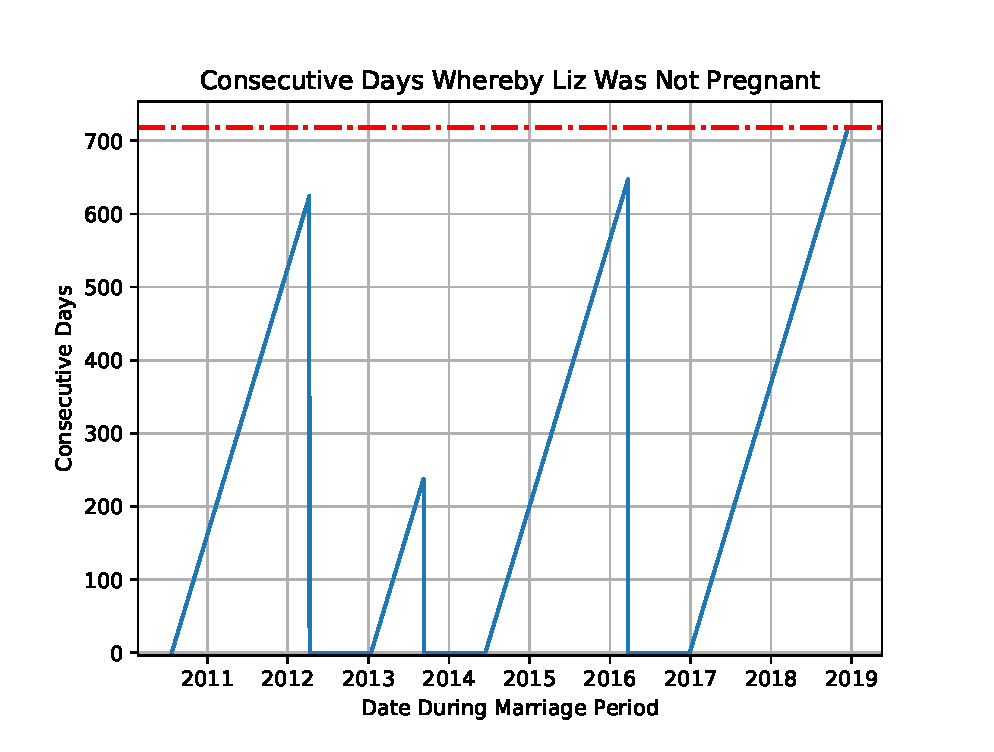
\includegraphics[angle=0]{plots/prego.eps}}
 \caption{Currently at marriage record duration for not being pregnant.}
\end{figurehere}

After a wonderful 8 years teaching in Johnston, Liz was able to land a
science teaching position in our hometown of Ankeny this school year. She is working
with 8th graders at Southview Middle School.  The new commute of 5 minutes
has proven beneficial given our children's ever expanding list of
activities.  Biking to work was seriously considered, but in the end she
decided to give it a year to settle in first.

The other 60% of our family is ignorant of minimum wage and happily does odd
jobs for shiny pennies.  Miss Maggie thought briefly that a dollar could be
worth 100 pennies, but the parents squashed that rebellion.

\section{Miss Charlotte}

Miss Charlotte's development has been fun to observe.  She presently knows many
words, but has yet to conjugate a sentence.  She was recently evicted from her
crib and into a standard issue twin bed.  Her wakeup routine is
to collect up all her blankeys, stuffed animals, and binkeys before heading
downstairs for breakfast.  Her stuffed animals are then arranged on the table
as shown by Figure 2.

%\bigskip

\begin{figurehere}
 \centering   
 \resizebox{.95\columnwidth}{!}{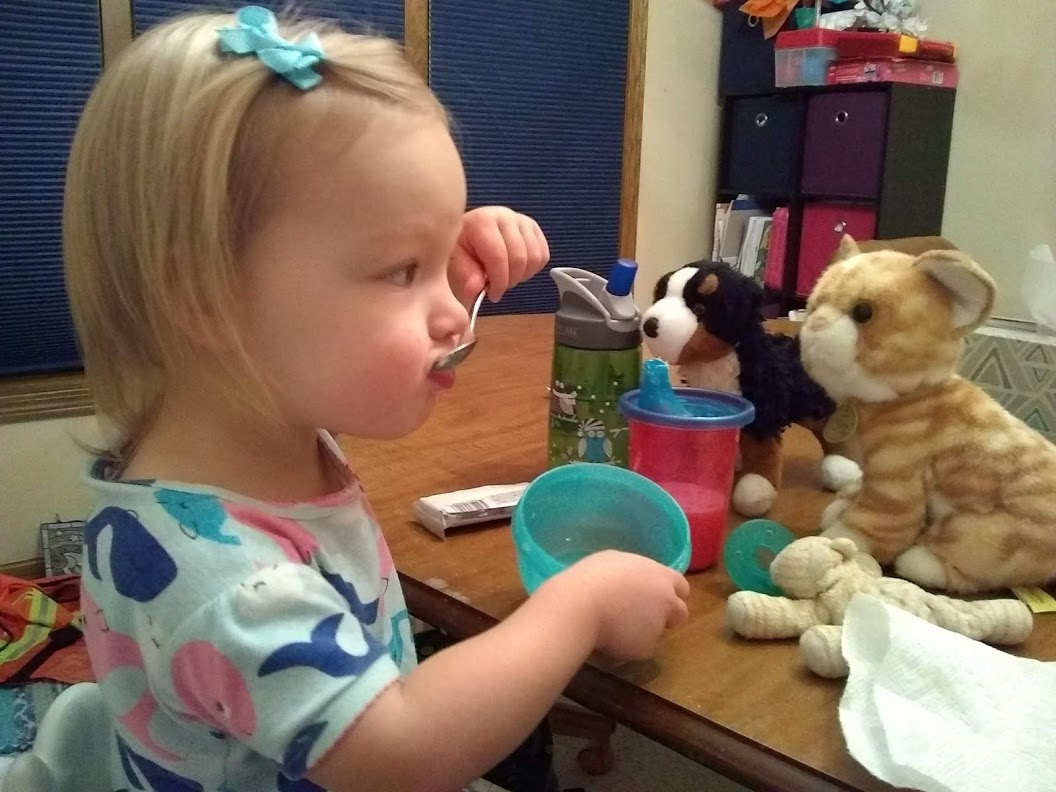
\includegraphics[angle=0]{plots/left.eps}}
 \caption{Charlotte eating breakfast with her left hand.}
\end{figurehere}

Miss Charlotte is an excellent eater, but now refuses most processed food
with prejudice.  She wants what the big people are having and her favorites
include noodles and bread.

\section{Mr Robert}

Mr Robert excels at generating entropy for this world.  He will play with
random toys for a few minutes, discard them to the side, find another toy to play with,
then complain when Miss Maggie plays with previously discarded toy.  He also
enjoys not smiling for various photoshoots (exception found with Figure 3), not
wishing to go to bed and then walking up before the rooster crows.  He is generally [[2132 Stevenson Dr]] a
good boy though and avoids getting into real trouble, at least to our knowledge.  He loves trains,
tractors, and trucks.

He took his sweet time to get potty trained, but finally made it.  Our advanced
methodology was to bribe him with \enquote{Marshmallow Cereal} (read Lucky
Charms).
Robert enjoys singing along at church and reciting prayers with a few second delay for
a nice echo effect to benefit others around us.

\section{Miss Maggie}

Miss Maggie is looking forward to starting kindergarten (Fall 2018).  We
are not exactly certain which school she will be attending yet, nor how the
logistics/finances will work out with her in school and the other two in
daycare.  She is starting to display \textit{Mother Hen} characteristics with
her younger siblings, but Iowa law forbids her from babysitting for us yet.  She is
excited to learn new vocabulary words each day and has started to figure out
how to read.  Her daddy's collection of Physics books are sure to be
voraciously consumed soon.

She enjoys coloring, inhaling ranch dressing with and without food, soccer, and
wrestling with daddy.  She has vacillated between future vocations of gardener,
school teacher, and astronaut.

\section{Summary}

It has been quite the year.  While the lack of sleep and fussing children can be
overwhelming at times, we are continually reminded of the many blessings and
great love within our family.  Seeing the children grow and do good deeds
without prodding is something we would not trade for all the sleep in the world.


\bigskip

\begin{figurehere}
 \centering   
 \resizebox{.95\columnwidth}{!}{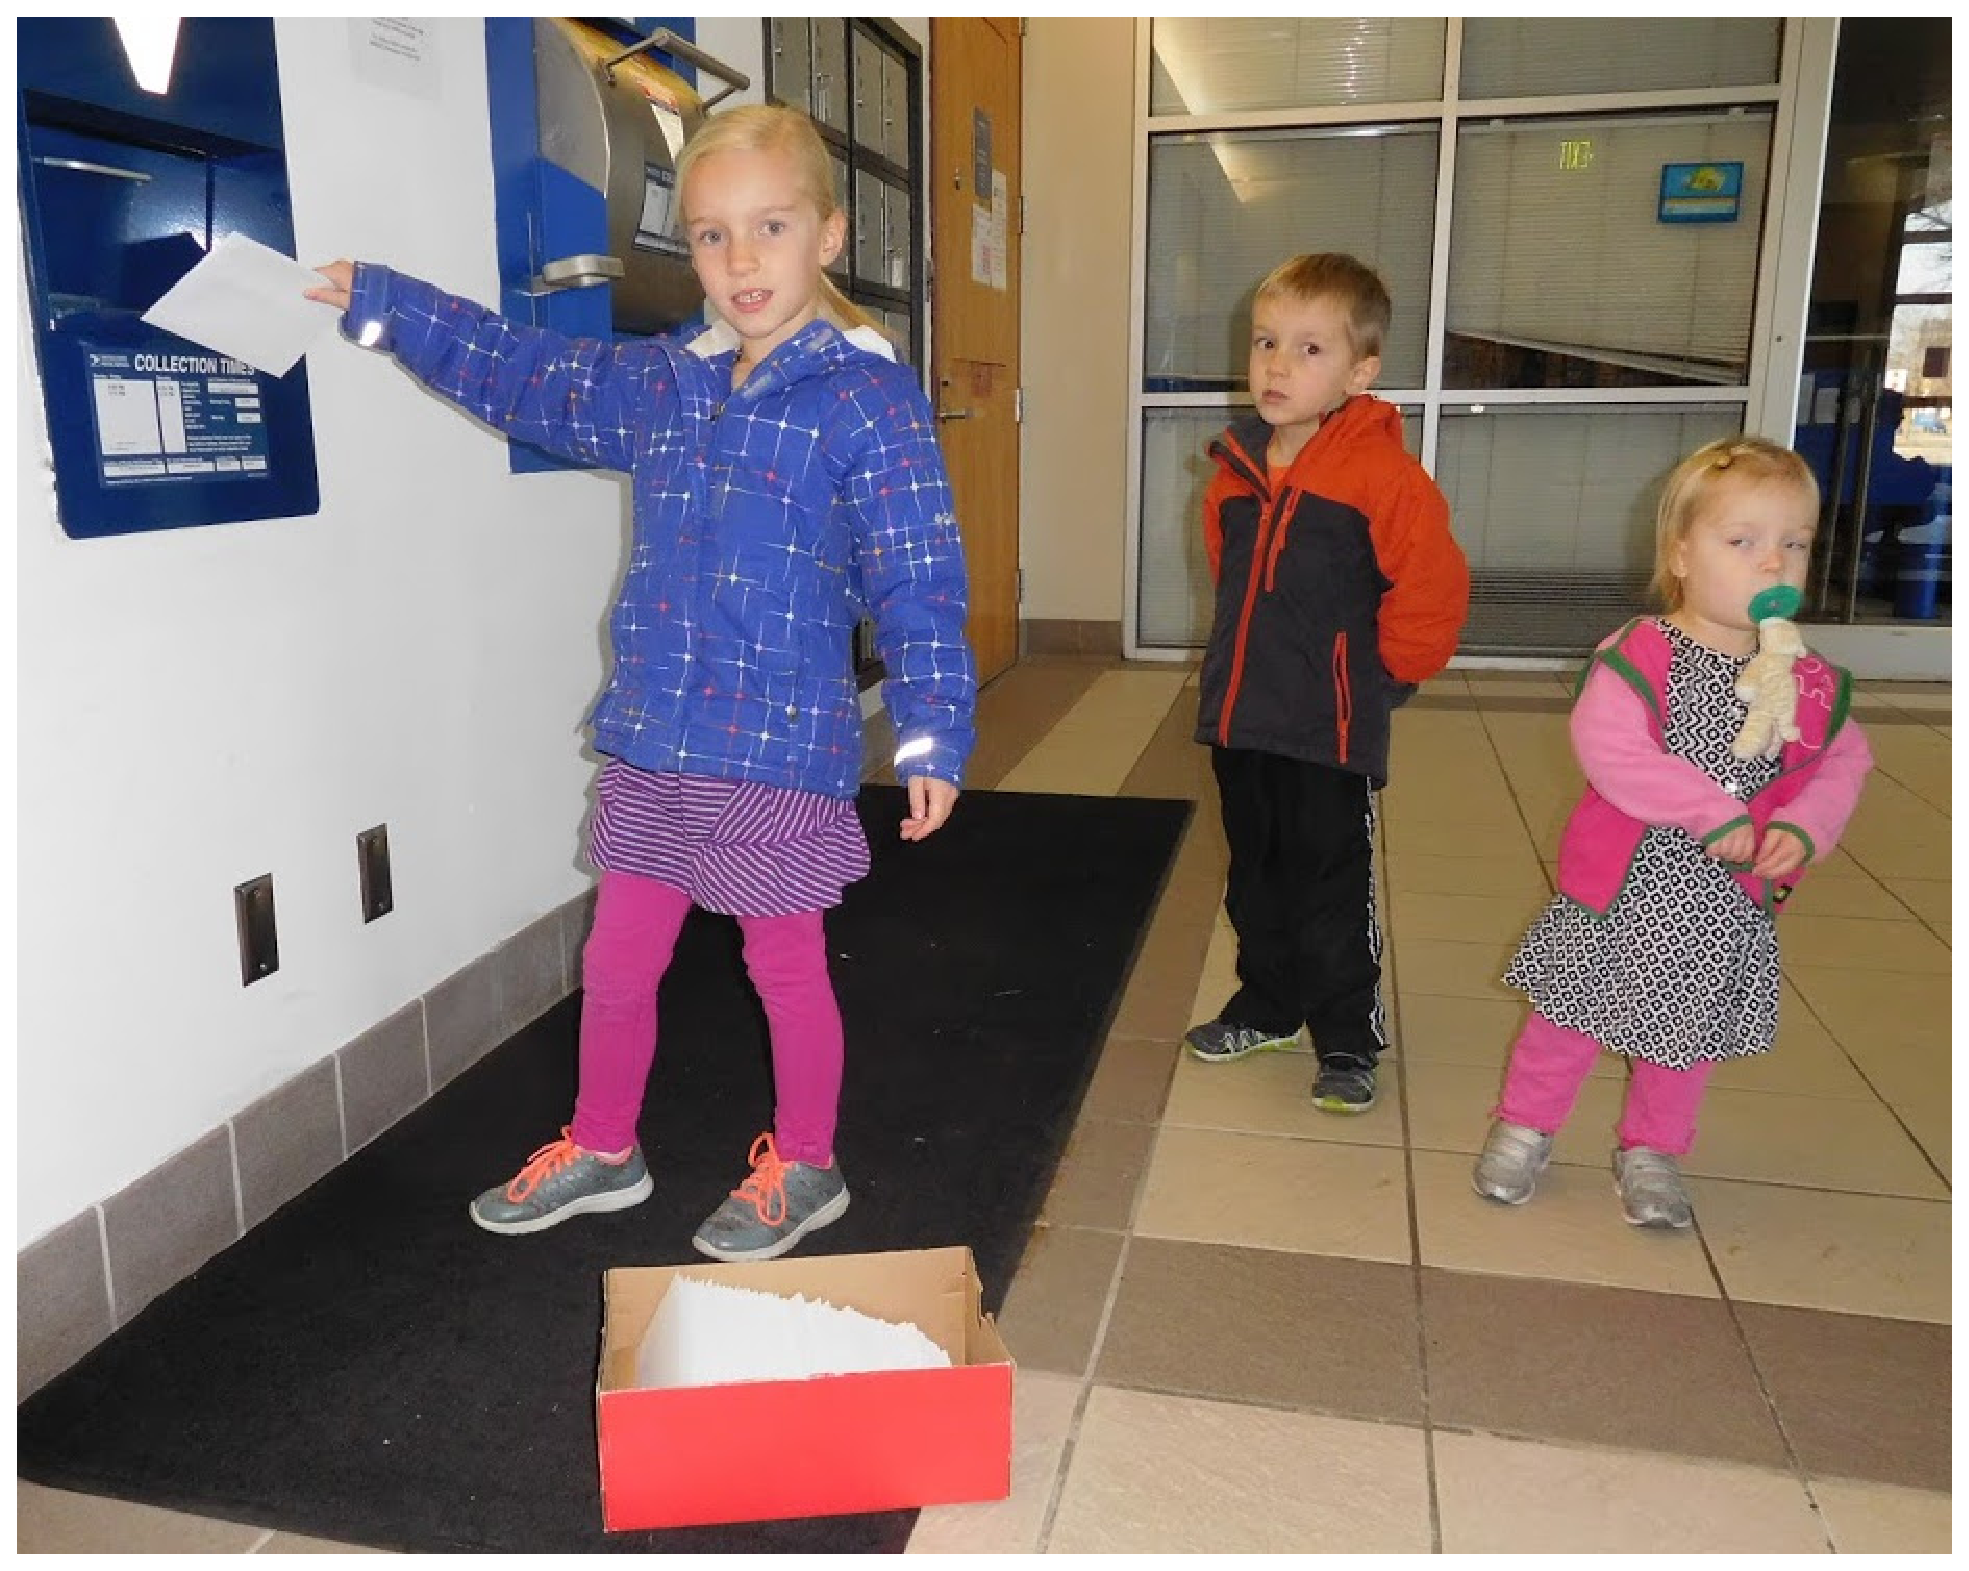
\includegraphics[angle=0]{plots/mail.eps}}
 \caption{The children delivering this year's letter to our local Amazon owned
 US Post Office. Miss Maggie thought it would be fun to place one letter at 
 a time into the receiver.}
\end{figurehere}

\bigskip
  \emph{Acknowledgments} Our family wishes to thank you for the generous 
support, prayers, cards, gifts, and visits you have provided us in the past
year. With your continued support, this letter will be produced again
next year. Please note that the format [[1431 E. 2nd]] chosen for this
correspondence was completely Daryl's idea and execution. Liz had marginal
editorial control. Full \LaTeX\xspace source can be found on Daryl's Github
page.

\section{References}

\refer Github, 2018: https://github.com/akrherz/me , visited 15 Dec 2018.
\refer Herzmann, Daryl E., et al. Herzmann Family Christmas Letter 2017. 

\end{multicols}

\end{document}

